\documentclass[
    10pt,
    aspectratio=169,
    xcolor={dvipsnames},
    spanish,
    % handout,
    % notes=only,
    % notes,
    ]{beamer}

% BEAMER SETTINGS
\setbeamerfont{section in toc}{size=\normalsize, shape=\bfseries}
\mode<presentation>{
    \usetheme{Antibes}
    \setbeamercovered{transparent}
    \usecolortheme{rose}
    \setbeamertemplate{navigation symbols}{}
    }
\useoutertheme{infolines}

% PACKAGES
% \usepackage[spanish]{babel}  % uncomment for Spanish support
\usepackage{tikz,pgfplots}
\pgfplotsset{compat=1.13}
\usetikzlibrary{calc}
\usepackage{subcaption}
\usepackage{graphicx}
\graphicspath{{figures}}
\usepackage{booktabs}
\usepackage{upgreek}
\usepackage{commath}
\usepackage{amsmath,amsthm,amssymb,mathtools,mathrsfs}
\usepackage{cancel}
\usepackage{fontawesome5}
\usepackage{enumerate}
\usepackage{tensor}
\usepackage[font=footnotesize]{caption}
\usepackage{wasysym}

\usepackage[skins,theorems]{tcolorbox}
\tcbset{
    highlight math style={
        enhanced,
        coltext=black,
        colframe=black,
        colback=lightgray,
        arc=0pt,
        boxrule=.5pt
        }
}

% REFERENCES AND OTHERS
\usepackage{aas_macros}
\usepackage{natbib}
\bibpunct{(}{)}{;}{a}{}{,}

\usepackage{siunitx}
\sisetup{
    range-phrase=\text{--},
    range-units=single,
    separate-uncertainty=true,
    print-unity-mantissa=false
    }
\DeclareSIUnit{\gauss}{G}
\DeclareSIUnit{\jansky}{Jy}
\renewcommand{\figurename}{Fig.}

\usepackage{hyperref}
\hypersetup{
    % bookmarks=true,
    unicode=true,
    pdftoolbar=true,
    pdfmenubar=true,
    pdffitwindow=false,
    pdfstartview={FitH},
    pdftitle={ISI-Free Linear Combination Pulses with Better Performanc},
    pdfauthor={Erik Saez A.},
    pdfcreator={Erik Saez A.},
    pdfnewwindow=true,
    colorlinks=true,
    linkcolor=RoyalBlue,
    citecolor=RoyalBlue,
    urlcolor=RoyalBlue
    }

\title[Auxiliar \#2 - Analisis de Sistemas dinamicos]{\bfseries Auxiliar \#2 - Analisis de Sistemas dinamicos}
\subtitle{}
\author[Erik Saez A.]{Erik Saez A.}
\institute[UChile]{Department of Electrical Engineering \\ Universidad de Chile}

\date{\today}

\begin{document}

\begin{frame}
  \titlepage
  \centering
  \faIcon{envelope} \href{mailto:erik.saez@ug.uchile.cl}{erik.saez@ug.uchile.cl} \hspace{.2cm}
\end{frame}

\begin{frame}
  \frametitle{Contenidos}
  \centering
  \begin{columns}
    \begin{column}{0.4\textwidth}
      \tableofcontents
    \end{column}
    \begin{column}{0.5\textwidth}
      \begin{figure}
        \centering
        
\includegraphics[width=\textwidth]{fcfm_die}
        \caption{Facultad de Ciencias Físicas y Matemáticas , Universidad de Chile.}
      \end{figure}
    \end{column}
  \end{columns}  
\end{frame}
%%%%%%%%%%%%%%%%%%%%%%%%%%%%%%%%%%%%%%%%%%

\section{Resumen de Conceptos}

\begin{frame}{Clasificación de Sistemas Dinámicos}
\begin{block}{Criterios de Clasificación}
  Los criterios de clasificacion de un sistema son maneras de \textbf{organizar y categorizar} los sistemas dinámicos en función de sus características y comportamientos.
  \footnotesize
  \begin{table}[h]
    \centering
    \begin{tabular}{|l|l|}
    \hline
    \textbf{Punto de vista} & \textbf{Clasificación} \\
    \hline
    Origen & Naturales - Artificiales \\
    \hline
    Naturaleza & Determinísticos - Aleatorios \\
    \hline
    Número de variables & Monovariables - Multivariables \\
    \hline
    Continuidad de variables & Variables discretas - continuas \\
    \hline
    Comportamiento espacial & Variables concentradas - distribuidas \\
    \hline
    Comportamiento temporal & Variable - Invariante \\
    \hline
    Linealidad de variables & Lineales - No lineales \\
    \hline
    Realizabilidad & Causales - Anticipativos \\
    \hline
    \end{tabular}
  \end{table}
\end{block}

\begin{alertblock}{Nota Importante}
  Una variable de estado puede convertirse en una variable de salida si se indica (existen variables de estado que no se pueden medir), por lo que la forma en que se designan las variables no es algo estático.
\end{alertblock}
\end{frame}

%%%%%%%%%%%%%%%%%%%%%%%%
%%%%%%%%%%%%%%%%%%%%%%%%
\begin{frame}{Análisis en Frecuencia}
\begin{block}{Introducción}
  \footnotesize
  Muchas veces el análisis de un sistema determinado se facilita si se realiza en función de su frecuencia, en vez del tiempo. Para esto existen distintas herramientas, tanto analíticas como computacionales, que sirven para distintos tipos de sistemas.
\end{block}

\begin{columns}
  \begin{column}{0.48\textwidth}
    \begin{block}{Transformada de Laplace}
      \footnotesize
      Se definen la transformada de Laplace unilateral y bilateral como:
      
      \textbf{Unilateral:} 
      $$\mathcal{L}\{f(t)\} = F(s) := \int_0^{\infty} f(t)e^{-st}dt$$
      
      \textbf{Bilateral:} 
      $$\mathcal{L}\{f(t)\} = F(s) := \int_{-\infty}^{\infty} f(t)e^{-st}dt$$
      
      donde $s = \sigma + j\omega$ es la "frecuencia compleja". Generalmente, las funciones resultantes de una transformada de Laplace se escriben con mayúsculas.
    \end{block}
  \end{column}
  
  \begin{column}{0.48\textwidth}
    \begin{block}{Propiedades Importantes}
      \footnotesize
      Esta transformada cumple con tres propiedades importantes:
      \begin{itemize}
        \item \textbf{Linealidad:} 
        $$\mathcal{L}\{af(t) + bg(t)\} = aF(s) + bG(s)$$
        \item \textbf{Desplazamiento:} 
        $$\mathcal{L}\{e^{at}f(t)\} = F(s-a)$$
        $$\mathcal{L}\{f(t-a)\} = e^{-as}F(s)$$
      \end{itemize}
    \end{block}
  \end{column}
\end{columns}
\end{frame}

%%%%%%%%%%%%%%%%%%%%%%%%
\begin{frame}{Análisis en Frecuencia}
\begin{block}{Definición}
  \footnotesize
  Una de las utilidades de la transformada de Laplace es que tiene una inversa:
  $$\mathcal{L}^{-1}\{F(s)\} = f(t) := \frac{1}{2\pi j} \int_{\sigma-j\infty}^{\sigma+j\infty} F(s)e^{st}ds$$
  Sin embargo, generalmente se usan tablas para calcular transformadas de Laplace y transformadas inversas, por lo que la forma analítica no resulta de mucha utilidad.
\end{block}

\begin{block}{Transformadas Básicas}
  \footnotesize
  \begin{itemize}
    \item $\mathcal{L}\{t^n f(t)\} = (-1)^n \frac{d^n}{ds^n} F(s)$
    \item $\mathcal{L}\{\delta(t)\} = 1$
    \item $\mathcal{L}\{(f * g)(t)\} = F(s)G(s)$
    \item $\mathcal{L}\{f^n(t)\} = s^n F(s) - s^{n-1}F(0) - s^{n-2}F'(0) - \cdots$
    \item $\mathcal{L}\left\{\int_0^t f(\tau)d\tau\right\} = \frac{F(s)}{s}$
    \item $F(s) = \frac{1}{1-e^{-sT}} \int_0^T f(s)e^{-st}dt$ si $f(t)$ $T$ periódica
  \end{itemize}
\end{block}
\end{frame}



%%%%%%%%%%%%%%%%%%%%%%%%
\section{Pregunta 1}
\begin{frame}{Pregunta \#1}
\begin{block}{Enunciado Pregunta \#1}
  \footnotesize
   Considere el sistema de la siguiente figura, donde se tiene un carro atado a un resorte con un sensor de distancia, capaz de medir la distancia del carro a la pared. Suponga que existe una fuerza de fricción viscosa con la superficie $F_f$ de la forma $F_f = b_1 \dot{z} + b_2 (\dot{z}^2)$.
    \begin{figure}[ht]
        \centering
        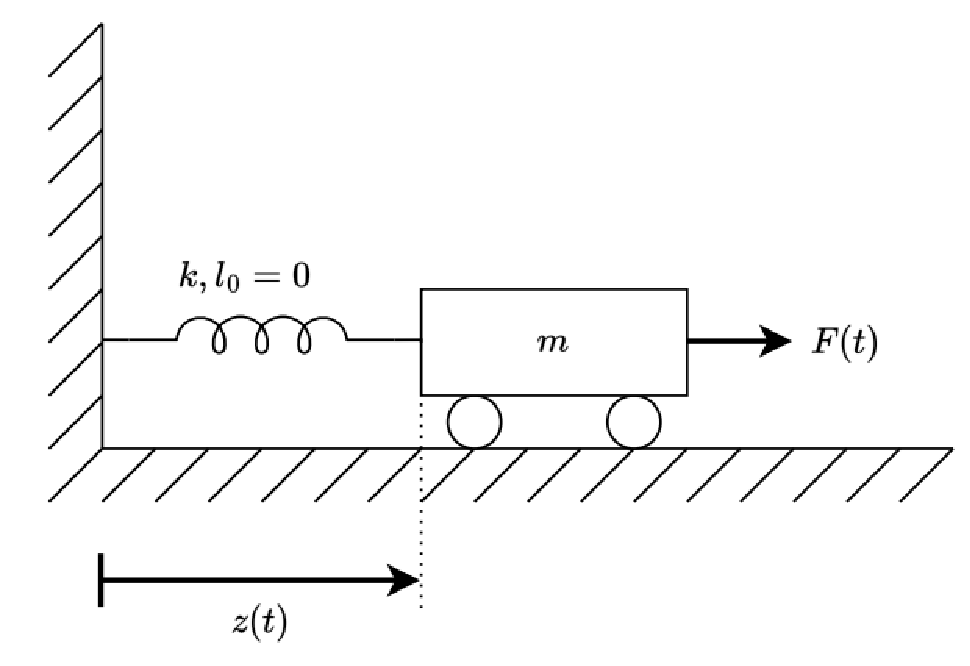
\includegraphics[width=0.3\textwidth]{Figura_2.pdf}
    \end{figure}
    \begin{enumerate}
        \item Establezca hipótesis simplificatorias para el problema.
        \item Formule un modelo matemático del sistema que sea consistente con sus hipótesis.
        \item Encuentre el punto de operación que asegure $z = 1$ m.
    \end{enumerate>
\end{block}
\end{frame>
%%%%%%%%%%%%%%%%%%%%%%
\section{Pregunta 2}
\begin{frame}{Pregunta \#2}
  \begin{block}{Enunciado Pregunta \#2}
  Considere el siguiente péndulo apoyado en un carro móvil, el cual se desliza por una barra.
    \begin{enumerate}
        \item Establezca hipótesis simplificatorias.
        \item Formule un modelo matemático, que capture la dinámica del sistema.
        \item Identifique entradas, salidas y estados en su modelo.
        \item Linealice en torno a $\theta = \pi$.
    \end{enumerate}
    \begin{figure}[ht]
        \centering
        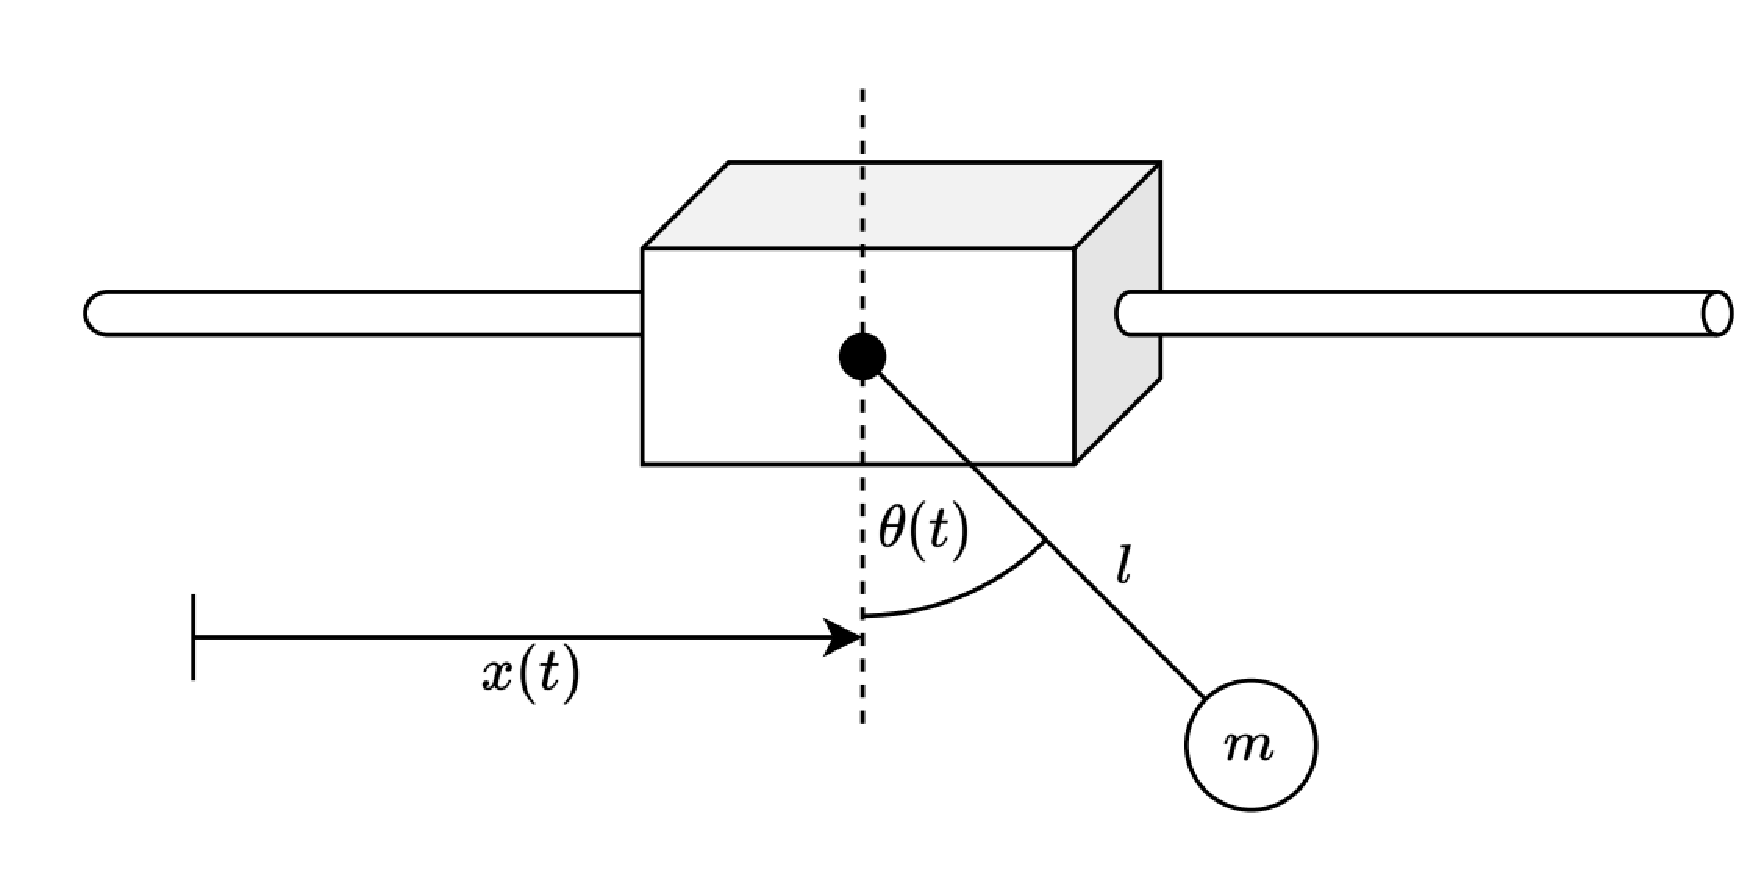
\includegraphics[width=0.4\textwidth]{Figura_3.pdf}
    \end{figure>
  \end{block}
\end{frame}

%%%%%%%%%%%%%%%%%%%%%%
\section{Pregunta 3}
\begin{frame}{Pregunta \#3: Estanque Cónico}
\vspace{-0.35cm}
\begin{columns}
    % Columna izquierda con figura y datos
    \begin{column}{0.34\textwidth}
      \vspace{-0.2cm}
      \begin{figure}[ht]
          \centering
          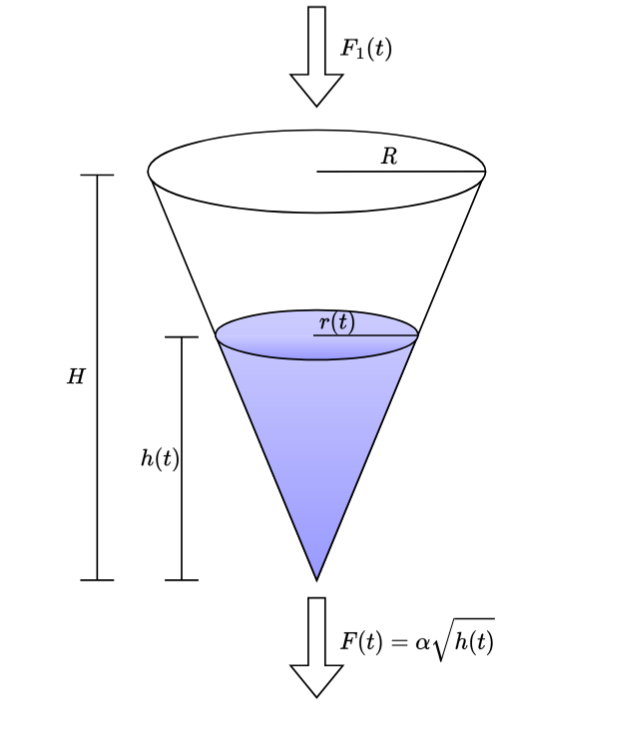
\includegraphics[width=0.63\textwidth]{Figura_4.png} % más pequeña
      \end{figure}
      \scriptsize
      \begin{block}{Datos del Sistema}
        \setlength\itemsep{0.1em}
        \begin{itemize}
            \item Altura máxima: $H = 8$ m
            \item Radio máximo: $R = 3$ m
            \item Volumen: $V(h) = \frac{\pi r^2 h}{3}$
            \item Flujo entrada: $F_1(t)$ (arbitrario)
            \item Flujo salida: $F(t) = \alpha \sqrt{h(t)}$, $\alpha = 1$
        \end{itemize}
      \end{block}
    \end{column}
    
    % Columna derecha con enunciado completo
    \begin{column}{0.64\textwidth}
      \scriptsize
      \begin{block}{Enunciado}
        Se tienen los siguientes datos y relaciones para el estanque cónico:
        \[
        V(h) = \frac{\pi r^2 h}{3}, \quad
        F(t) = \alpha \sqrt{h(t)}, \quad \alpha = 1
        \]
        \textbf{Responda lo siguiente:}
        \begin{enumerate}
            \setlength\itemsep{0.2em}
            \item Encuentre un modelo dinámico no lineal que relacione $h(t)$ y $F_1(t)$, indicando claramente las hipótesis simplificatorias.
            \item Linealice su modelo en torno a $h_0 = 4$ m, $F_{1,0} = 2$ m³/s, para el modelo perturbado:
            \[
                h(t) = h_0 + \Delta h(t), \quad 
                F_1(t) = F_{1,0} + \Delta F_1(t)
            \]
            que relacione la salida $\Delta h(t)$ con la entrada $\Delta F_1(t)$, despreciando términos de orden superior.
        \end{enumerate}
      \end{block}
    \end{column}
  \end{columns}
\end{frame}

\end{document}
